\documentclass[a4paper,11pt,english]{book}
\usepackage[english]{babel}
\usepackage{listingsutf8,verbatim} %inclure du code 
\lstloadlanguages{R}
\usepackage[utf8]{inputenc} % Required for including letters with accents
\usepackage[T1]{fontenc} % Use 8-bit encoding that has 256 glyphs
\usepackage[dvipsnames]{xcolor}
\usepackage{xspace}
\usepackage{graphicx,epsfig,subfigure}
\usepackage{ragged2e}
\usepackage{fancyhdr}
\usepackage{booktabs}
\fancyhead[L]{
\includegraphics [width=1cm]{images/Logo_ponts_paristech}}
\fancyhead[R]{\leftmark}
\usepackage[left=3.5cm,right=3.5cm,top=4.5cm,bottom=5.0cm]{geometry}  % Page margins
\usepackage{eso-pic}
\usepackage[Glenn]{fncychap}
\usepackage{array,supertabular,amsmath,amssymb,dsfont}
\usepackage{stmaryrd}
\usepackage{titlesec}
\usepackage{tablefootnote}
\usepackage{multicol,array}
\usepackage{float}
\usepackage{color}
\usepackage[most]{tcolorbox}
\usepackage{pgfplots}
  \pgfplotsset{compat=1.13}
\usepackage{xcolor}
\newcommand\BackgroundPic{%
\put(0,0){%
\parbox[b][\paperheight]{\paperwidth}{%
\vfill
\centering
\includegraphics[width=\paperwidth,height=\paperheight,%
keepaspectratio]{background.jpg}%
\vfill
}}}
\setlength\belowcaptionskip{0.3cm}
\setlength\abovecaptionskip{0.3cm}
\usepackage[hang,small]{caption}
\usepackage{subfigure}
\usepackage{subcaption}
\usepackage{multirow} 
\usepackage{multicol}
\usepackage{colortbl}
\usepackage[demo]{graphicx}
\usepackage{textcomp,eurosym} 
\setlength{\headheight}{36.06802pt}
\renewcommand{\footrulewidth}{0.4pt}
\renewcommand{\headrulewidth}{0.4pt}
\fancyhead[R]{\leftmark}
\renewcommand{\arraystretch}{1.2} %aérer tableaux 
\definecolor{dkgreen}{rgb}{0,0.6,0}
\definecolor{gray}{rgb}{0.5,0.5,0.5}
\definecolor{mauve}{rgb}{0.58,0,0.82}
\usepackage{stmaryrd} %double crochet
\usepackage{amsthm}
\usepackage{mathrsfs,amsmath} 
\newtheorem{prop}{Proposition}
\newtheorem*{theorem}{Théorème}
\usepackage[left=3.0cm,right=3.0cm,top=5.5cm,bottom=5.5cm]{geometry} % Page margins
\usepackage[colorlinks=true,urlcolor=blue,linkcolor=blue]{hyperref}
\let\cleardoublepage\clearpage
\definecolor{ballblue}{rgb}{0.13, 0.67, 0.8}
\definecolor{orange}{RGB}{242,239,121}
\definecolor{darkorange}{RGB}{229,186,27}
\linespread{1.05}
\newcommand{\Lim}[1]{\raisebox{0ex}{\scalebox{1}{$\displaystyle \lim_{#1}\;$}}}
\usepackage{longtable}
\usepackage{etoolbox,siunitx}
\usepackage{tabularx}
\newrobustcmd*{\bftabnum}{%
  \bfseries
  \sisetup{output-decimal-marker={\textmd{.}}}%
}
\usepackage{rotating}
\usepackage{collcell}

\newcommand{\setmaxnum}[1]{%
    \gdef\maxnum{#1}%
}
\newcommand{\numtest}[1]{%
    \ifdim#1pt > \maxnum pt
        $\mathbf{#1}$%
    \else
        $#1$%
    \fi%
}
\newcolumntype{E}{>{\collectcell\numtest}r<{\endcollectcell}}

\begin{document}
\sisetup{detect-weight=true,detect-inline-weight=math}

\frontmatter
%----------------------------------------------------------------------------------------
%	TITLE PAGE
%----------------------------------------------------------------------------------------
\begin{titlepage}
\begin{center}
\begin{figure}[H] 
  %\begin{minipage}[b]{0.5\linewidth}
    \centering
    
\includegraphics[scale=0.2]{images/Logo_ponts_paristech.png} 
    \vspace{4ex}
  %\end{minipage}
\end{figure}
% Title
\rule{\linewidth}{0.5mm} \\[0.4cm]
{ \LARGE \bfseries Pricing Callable Barrier Reverse Convertibles with a Reflected Forward-Backward Stochastic Differential Equations System \\
}
\rule{\linewidth}{0.5mm} \\[1cm]


Caroline \textsc{OSTER}

\noindent

\vspace{4cm}

{\today}
\end{center}
\end{titlepage}
\newpage

\pagestyle{empty}
\tableofcontents
\listoffigures
\listoftables

%--------------------------------------------------------------------------
%	Intro
%--------------------------------------------------------------------------
\mainmatter
\chapter*{Introduction}
\addcontentsline{toc}{chapter}{Introduction}
\vspace*{-2cm}

Structured products represent an attractive alternative to classical securities and direct investments such as bonds, equities, commodities etc. Issued by a bank or an insurance company, they are generally composed of 2 elements, one ensuring the capital protection, and one boosting the yield. They were created to meet specific needs and can be used to reduce, mitigate and control the risks of a portfolio. In Switzerland, markets are particularly driven by structured products with CHF 190 billions invested in those kinds of securities at Swiss banks, which makes about 5\% of the total assets managed in the country \cite{SSPA}.

In this report, we will focus on a particular structured product called Barrier Reverse Convertible (BRC). A BRC is a kind of reverse convertible security linked to an underlying stock that can be either an equity index or a basket of indices. The capital repayment is made at maturity ; it can be 100\% of the principal if the underlying stock has not reached a predetermined barrier and less otherwise. A BRC also pays highly-rated coupons that enhance the attractiveness of the product.

Reverse convertible securities are among the most popular products in Switzerland in terms of risk-optimization, especially if the investor expects the market to move upward. In order to illustrate that, we present in Figure \ref{fig:median-returns-BRC} the median returns of Swiss BRCs p.a. from 2008 to 2014 \cite{SSPA-study} and compare it with the evolution of the SMI index during the same period\footnote{We use this index as a proxy for the Swiss market.}. We can see that the median return of the BRCs seems effectively to be positively correlated with the index trend. As the volatility is generally decreasing with the stock price getting higher, this could also mean that someone investing in a BRC would expect lower volatility in the future. The mechanisms hidden behind those observations will be better explained further in this report.

\begin{figure}[H] 
    \centering
    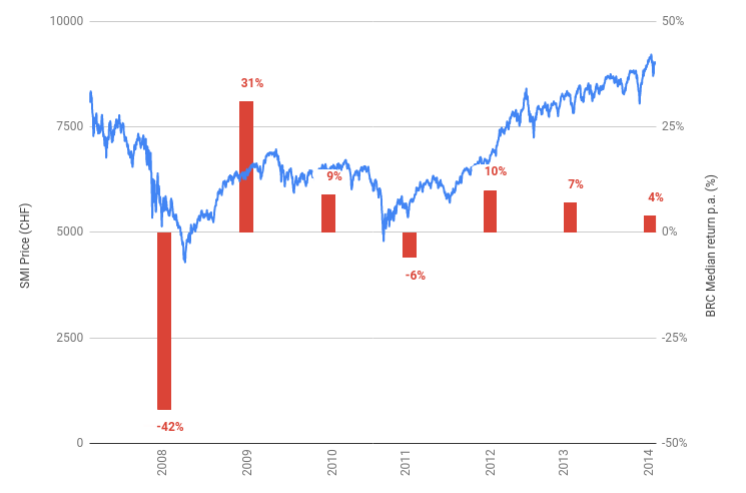
\includegraphics[scale=0.4]{images/BRC_median_return.png} 
    \caption{BRC median returns in \% in Switzerland compared with the SMI index evolution}
    \label{fig:median-returns-BRC}
\end{figure}

The main objective of this report is the pricing of a Barrier Reverse Convertible with a possibility to be called by the issuer at certain dates precised in the contract. Indeed, this kind of particularity brings a complexity to the product that prevents from pricing with a basic Monte Carlo methodology. We thus considered the problem in a backward manner and used a system of reflected forward-backward stochastic differential equations to model and compute the price. The pricing has been made under the Black-Scholes model and the no-arbitrage assumption, which is easily manageable with the modeling chosen and provides rather good performances in terms of accuracy and velocity of the convergence. \\

First will be introduced the exact definition of a callable BRC, and then the pricing methodology used for this asset. Finally we will present our results and some possible extensions we considered.  



%--------------------------------------------------------------------------
%	Chapter 1 
%--------------------------------------------------------------------------

\pagestyle{fancy}

\chapter{Description of a callable barrier reverse convertible}

\section{Definition of a Standard Reverse Convertible}
In order to understand what a Barrier Reverse Convertible is, we will first give a brief definition of a Standard Reverse Convertible : this kind of financial instrument is a bond-like security which pays a coupon that is generally very high compared to the risk-free interest rate. This bond is combined with a short put option, as can be seen in \ref{fig:RC-payoff}.

\begin{figure}[!h]
    \centering
    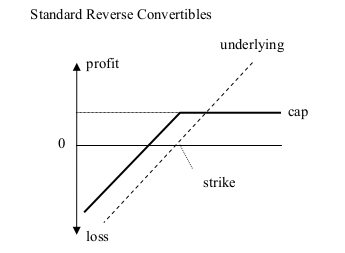
\includegraphics[scale=0.7]{images/RC.png}
    \caption{Payoff profile of a \textit{Reverse Convertible}. Source : \cite{lindauer2008pricing}}
    \label{fig:RC-payoff}
\end{figure}

The payment is made as follows : if the price of the underlying ends above the strike at maturity, the nominal is given back as the final payoff. In this case, the final payoff is called the cap. On the contrary, if the price of the underlying ends under the strike at maturity, the final payoff is the cap reduced by the difference between the strike and the final price. All the coupons are paid during the lifetime of the asset.\\

Let us denote $K$ the strike of the asset and $S_{T}$ the price of the underlying at maturity $T$. The final payoff $P$ can hence been expressed as follows :
$P=\text{cap}-(K-S_{T})_{+}$.\\

With this kind of security, the investor generally expects the market to move higher or at least to remain stable, so he doesn't lose his capital and makes benefits with high coupons. Moreover, a Reverse Convertible can be beneficial if the volatility is expected to decrease or to stay low in the future, as the investor is mainly shorting volatility.

\section{Definition of a Barrier Reverse Convertible}
\label{sec:BRC-definition}

The Barrier Reverse Convertible is slightly different because it contains a barrier on the level of the underlying : if the underlying doesn't reach the barrier during the lifetime of the asset, the nominal is given back at the end, but in the case it is, the put is activated and the final payoff is the one of a short put. Of course, coupons are paid according to the terms of the contract. The main difference with the Reverse Convertible is thus the path-dependency of the asset. \\

Figure \ref{fig:BRC-payoff} summarizes the payoff profile of a Barrier Reverse Convertible:

\begin{figure}[!h]
    \centering
    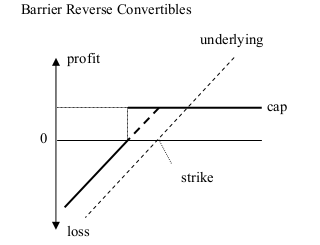
\includegraphics[scale=0.65]{images/BRC.png}
    \caption{Payoff profile of a \textit{Barrier Reverse Convertible}. Source : \cite{lindauer2008pricing}}
    \label{fig:BRC-payoff}
\end{figure}

The barrier is always a knock-in option\footnote{See Appendix \ref{appendix:down-in-put} for a reminder on barrier options}, but it can be either 'up' or 'down'. If the barrier is 'up', it means that it is reached if the level of the underlying is above it. If the barrier is down, it is reached if the level of the underlying is below it.

\section{Multi Barrier Reverse Convertibles}
\label{sec:multi-BRC-definition}
Multi \textit{Barrier Reverse Convertibles} are a type of Barrier Reverse Convertibles that have several underlyings. This changes the definition of how the barrier is reached and if the final value is above the strike. In both aspects, several definition can be considered :

\begin{itemize}
    \item \textbf{"WorstOf" case}: in this case, the underlying chosen to be compared with the barrier (or the strike) is the one with the worst performance regarding the barrier (or the strike).
    \item \textbf{"BestOf" case}: in this case, the underlying chosen to be compared with the barrier (or the strike) is the one with the best performance regarding the barrier (or the strike).
    \item \textbf{"Basket" case}: in this case, a linear combination of the performances of the underlyings is chosen to be compared with the barrier (or the strike).
\end{itemize}

The choice of the underlying to be compared with the barrier can be different from the one to be compared with the strike, which allows 9 different types of multi BRCs.

\section{Adding the callability}
To the regular (multi) BRCs can be added the callability by the issuer. This means that the issuer can buy the contract at several dates and at a certain amount specified in the contract. The amount of this redemption is generally the nominal plus the on-going coupon.

%--------------------------------------------------------------------------
%	Chapter 2 
%--------------------------------------------------------------------------

\pagestyle{fancy}

\chapter{Pricing Methodology}
\label{chap:pricing-methodology}
Since the financial instrument we want to price is a multi-dimensional asset, the best choice of pricing methodology seems to be a Monte Carlo method. The only problem with it is that the price between the beginning and the maturity of the contract is unknown, and more particularly at the times of possible redemption by the issuer (called times of callability). But the price of the asset at those particular times has to be known (and compared with the amount of redemption precised in the contract) in order to determine whether the callability is activated or not by the issuer. A first and naive idea would be to use a new Monte Carlo at each time step needed, but this would be computationally too long and too complex to be efficient.  

A better solution would be to proceed in a backward manner, beginning with the price at maturity (which is known thanks to the explicit final payoff profile) and coming back to the price at $t=0$ step by step. With this approach, inspired by the Longstaff-Swartz algorithm \cite{schwartz2001valuing}, the price can be known at all the possible redemption times.

Hence, the modeling chosen here is a forward-backward stochastic differential equation system. The forward component, which only represents the diffusion of the underlyings, will be resolved in a classical way whereas solving the backward component will allow us to compute the price, taking into account the coupons and the callability at each time step.

The whole methodology will be described in this chapter. First, we will present the modeling chosen to solve the problem considered, and justify the hypothesis made within this context. Then will be explained the forward equation resolution, the final payoff computation and the computation of the price in a backward manner.


\section{Presentation of the SDE system}
\label{sec:SDE-presentation}
As explained above, the objective is to compute the solution of  a forward-backward stochastic differential equation (FBSDE) which can be written as follow :
$$S_{t} = S_{0}+\int_{0}^{t}b(s,S_{s})ds +\int_{0}^{t} \sigma(s,S_{s})dW_{s}$$
$$Y_{t} = \Phi(\textbf{S}) + \int_{t}^{T}f(s,Y_{s},Z_{s})ds -\int_{t}^{T}Z_{s}dW_{s}$$
$\textbf{S}=(S_{t})_{t\geq0}$ is the forward component of the system. It represents the underlyings and its dimension is $d$. $(Y_{t})_{t\geq0}$ represents the value of a replicating portfolio at time t and is uni-dimensional.\\
The process $W$ is a d-dimensional brownian motion defined on a probability space $(\Omega,\mathcal{F},\mathbb{P})$ provided with its natural filtration $(\mathcal{F)}_{t}$ and generated by $W$. 
$T$ is the maturity of our asset.\\

The function $f$ is called the driver function. It should be uniformly Lipschitz, \textit{ie} there exist a constant $C$ such that :
$$\forall (y_{1},z_{1}),(y_{2},z_{2}), |f(t,y_{1},z_{1})-f(t,y_{2},z_{2})|\leq C(|y_{1}-y_{2}|+|z_{1}-z_{2}|)$$

Antonelli \cite{antonelli1993backward} proved the existence of such a solution using a fixed point theorem when the function $b$ does not depend on $(Z_{t})_{t\geq0}$ (which is our case) and under the condition $CT<1$ with $C$ the Lipschitz constant of $f$. In our case, $C$ is the risk free rate (see \ref{subsec:choice-of-f}); it is small enough so that this condition is almost always verified.\\

Resolving the backward equation thus consists in computing a pair of processes $(Y,Z)$. We will more especially focus on the process $(Y_{t})_{t\geq0}$ which gives the price of the option.

\section{Resolution of the forward equation}
\subsection{Model and scheme of discretization for the underlyings}
\label{subsec:underlying-discretization}
The model used for the diffusion of the underlyings is the Black-Scholes model. As the pricing is done under risk-neutral probability, we have for each underlying $(S^{i}_{t})_{t\geq0}$:
$$
\begin{cases}
dS_{t}^{i}=r\text{d}t+\sigma_{i}\text{d}W_{t}^{i} \\
S_{0}^{i}=s_{0}^{i} 
\end{cases}
$$
where $r$ is the risk free rate.
If we take a time grid $(t_{0},t_{1},\ldots,t_{m})$, we know that the solution of that stochastic equation can be discretized as follows :
$$\begin{cases}
\forall k=1,\ldots,m,  S_{t_{k}}^{i}=S_{t_{k-1}}^{i}e^{(r-\frac{\sigma_{i}^{2}}{2})(t_{k}-t_{k-1})+\sigma_{i}W_{t_{k}}^{i}}\\
S_{t_{0}}^{i}=s_{0}^{i} 
\end{cases}
$$
with $W_{t_{k}}^{i} \sim \mathcal{N}(0,t_{k}-t_{k-1})$.\\

\subsection{Taking into account the correlation}
Moreover, the brownian motions are all correlated : $$\forall (i,j) \in \{1,\ldots,d\}\times\{1,\ldots,d\},~ \mathbb{E}(\text{d}W_{t}^{i}\text{d}W_{t}^{j})=\rho_{ij}\text{d}t$$
In order to take into account these correlations, we should generate the brownian motions with a multivariate Gaussian distribution with correlation matrix $\Sigma=(\rho_{i,j})_{(i,j) \in \{1,\ldots,d\}\times\{1,\ldots,d\}}$.\\

The first step is to generate $d$ independent realizations of a standard normal distribution in a matrix $M$. Then, we should calculate the matrix $C$ such that $CC^{T}=\Sigma$ thanks to a Cholesky decomposition. To do so, the matrix $\Sigma$ has to be definitive positive, which is not always the case. \\

\begin{tcolorbox}[breakable,colback=cyan,opacityfill=0.05,colframe=blue,width=\dimexpr\textwidth+12mm\relax,enlarge left by=-6mm]
\begin{center}
\vspace{0.2cm}
\textbf{How to make a matrix $\Sigma$ definite positive ?}
\end{center}
\begin{enumerate}
    \item Diagonalize the matrix $\Sigma$, \textit{ie} find $P$ an invertible matrix and $D$ a diagonal matrix such that $\Sigma=PDP^{-1}$
    \item Let $(d_{ii})_{i \in \{1,\ldots,d\}}$ be the diagonal elements of the matrix $D$. We calculate : $$\forall i=1,\ldots,d, d_{ii}^{*}=\begin{cases}
        d_{ii}& \text{ if } d_{ii}>0 \\
        10^{-12}& \text{ if } d_{ii}\leq0
    \end{cases}$$
 \item Writing $D^{*}$ the diagonal matrix with $d_{ii}^{*}$ the diagonal elements, we can compute $$\Sigma^{*}=PD^{*}P^{-1}$$ where $\Sigma^{*}$ is the corrected definite positive matrix.
\end{enumerate}
\end{tcolorbox}
Once the matrix $C$ is computed, we can calculate the matrix $Z=CM$ which gives a realization of a multivariate Gaussian distribution whose correlation matrix is $\Sigma$.
\subsection{Brownian bridge and final payoff computation}
\label{subsec:brownian-bridge}
The problem of the discretization of the forward equation is that we lose the continuous monitoring of the BRC's barrier. In order to catch the continuity of the barrier without using a very high number of steps in the time grid, we decided to use brownian bridges.\\

Let's first reason with only one underlying $(S_{t})_{t\geq0}$ of volatility $\sigma$. The probability to reach down the barrier $B$ between $t_{k}$ and $t_{k+1}$, knowing that $S_{t_{k}}=x$ and $S_{t_{k+1}}=y$, is given by \footnote{See Appendix \ref{appendix:brownian-bridge} for the demonstration of this formula}:
$$p(x,y,t_{k+1}-t_k,B,\sigma) = 
\begin{cases}
1 &\text{ if } x\leq B \text{ or } y\leq B \\
\exp(-2\frac{\log(\frac{x}{B})\log(\frac{y}{B})}{\sigma^{2}(t_{k+1}-t_k)}) &\text{ otherwise }
\end{cases}$$
The probability that the underlying has not touched the barrier during the whole lifetime of the asset is then $p=\prod_{i=1}^{m}(1-p_{i})$ where $p_{i}=p(S_{t_{i}},S_{t_{i+1}},(t_{i+1}-t_i),B,\sigma_{i})$. When computing the payoff, one has to take into account this probability as follows :
$$\Phi(S) = \text{cap} -(K-S_{T})_{+}(1-p)$$

When it comes to several underlyings, the computation of $p$ becomes harder. As explained in \ref{sec:multi-BRC-definition}, the barrier can be a \textit{WorstOf} or a \textit{BestOf}. This means that there exists 4 cases :
\begin{enumerate}
    \item \textbf{The barrier is a \textit{WorstOf} and is down} : the barrier is touched if at least one of the underlying has touched the barrier, which is the complementary of the event "Not any underlying has touched the barrier". We then have $p_{i}=1-\prod_{j=1}^{d}(1-p_{i}^{j})$, where $p_{i}^{j}$ is the probability that the $j^{th}$ underlying has reached the barrier between $t_{i}$ and $t_{i+1}$.
    
    \item \textbf{The barrier is a \textit{WorstOf} and is up} : the barrier is touched if all the underlyings have, thus $p_{i}=\prod_{j=1}^{d}p_{i}^{j}$
    
    \item \textbf{The barrier is a \textit{BestOf} and is down} : this situation is the same as above, so we have $p_{i}=\prod_{j=1}^{d}p_{i}^{j}$
    
    \item \textbf{The barrier is a \textit{BestOf} and is up} : this situation is the same as the first one so  $p_{i}=1-\prod_{j=1}^{d}(1-p_{i}^{j})$
\end{enumerate}
Note that in order to compute those probabilities, we have made the strong assumption of independence between the different underlyings, which is not really the case. Nevertheless, this approximation is necessary to have simple formulas and to take them into account in the payoff computation.
\section{Resolution of the backward equation}
\subsection{Choice of the function f}
\label{subsec:choice-of-f}
In order to find the expression of $f$ and to give more intuition about what the process $(Z_{t})_{t\geq0}$ represents, we set up a self-financing portfolio $Y_{t}$ and buy $a_{t}$ stocks $S_{t}$ at time $t$. The rest of the portfolio is invested in a bond whose risk-free rate is $r$. The value of the portfolio should then evolve like this :
$$dY_{t} = r(Y_{t}-a_{t}S_{t})\text{d}t + a_{t}dS_{t}$$
$$dY_{t} = r(Y_{t}-a_{t}S_{t})\text{d}t + a_{t}(rS_{t}\text{d}t+\sigma S_{t}\text{d}W_{t})$$
We can rewrite this :
$$dY_{t} = rY_{t}\text{d}t + \sigma a_{t}S_{t}\text{d}W_{t}$$
The process $(Y_{t})_{t\geq0}$ presented in \ref{sec:SDE-presentation} is a solution of this SDE with $f(t,Y_{t})=-rY_{t}$, $Z_{t} = \sigma a_{t}S_{t}$ and the terminal condition $\Phi(S)=Y_{T}$.
The hedging-strategy corresponds to $Z_{t}=\sigma S_{t} a_{t}$ where $a_{t}$ is the $\Delta$ of the option. 
\subsection{Resolution formula}
Let us rewrite the backward equation at $t_{k}$ and $t_{k+1}$, two consecutive times in the time grid :
$$Y_{t_{k}} = \Phi(S) + \int_{t_{k}}^{T} f(s,Y_{s}) ds - \int_{t_{k}}^{T} Z_{s} dW_{s}$$
$$Y_{t_{k+1}} = \Phi(S) + \int_{t_{k+1}}^{T} f(s,Y_{s}) ds - \int_{t_{k+1}}^{T} Z_{s} dW_{s}$$
Now let's make the difference between both :
\begin{equation}
    Y_{t_{k}} = Y_{t_{k+1}} + \int_{t_{k}}^{t_{k+1}} f(s,Y_{s}) ds - \int_{t_{k}}^{t_{k+1}}Z_{s} dW_{s}
    \label{eq:Y_t}
\end{equation}
Let $(\mathcal{F}_{t})_{t\geq0}$ be a filtration so that $(Y_{t})_{t\geq0}$ and $(S_{t})_{t\geq0}$ are adapted, and let's apply $\mathbb{E}(.|\mathcal{F}_{t_{k}})$ to the previous equation :
$$\mathbb{E}(Y_{t_{k}}|\mathcal{F}_{t_{k}}) = \mathbb{E}(Y_{t_{k+1}}|\mathcal{F}_{t_{k}}) + \mathbb{E}\left(\int_{t_{k}}^{t_{k+1}} f(s,Y_{s}) ds~\bigg\vert~\mathcal{F}_{t_{k}}\right) - \mathbb{E}\left(\int_{t_{k}}^{t_{k+1}}Z_{s} dW_{s}~\bigg\vert~\mathcal{F}_{t_{k}}\right)$$

The last term is equal to zero because $\mathbb{E}(\int_{t_{k}}^{t_{k+1}}Z_{s} dW_{s}|\mathcal{F}_{t_{k}})=\mathbb{E}(\int_{t_{k}}^{t_{k+1}}Z_{s} dW_{s})$ thanks to the independence, and $\mathbb{E}(\int_{t_{k}}^{t_{k+1}}Z_{s} dW_{s})=0$ as being the expectation of an Ito's integral.\\
For the deterministic term, we have $\mathbb{E}(\int_{t_{k}}^{t_{k+1}}f(s,Y_{s}) ds|\mathcal{F}_{t_{k}})=\mathbb{E}(\int_{t_{k}}^{t_{k+1}}f(s,Y_{s}) ds) = \int_{t_{k}}^{t_{k+1}}f(s,Y_{s}) ds$.
We thus have :
\begin{equation}
    Y_t = \mathbb{E}(Y_{t_{k+1}}|\mathcal{F}_{t_{k}}) + \int_{t_{k}}^{t_{k+1}}f(s,Y_{s}) ds
\end{equation}
Let us denote $\Delta_{k}=t_{k+1}-t_{k}$. We will consider the following approximation for the integral :
$$\int_{t_{k}}^{t_{k+1}}f(s,Y_{s})ds \simeq \Delta_{t_{k}}\theta f(t_{k},Y_{t_{k}}) + \Delta_{t_{k}}(1-\theta) f(t_{k+1},Y_{t_{k+1}})$$
and choose $\theta=1$. The resolution formula becomes :
\begin{equation}
Y_{t_{k}} = \mathbb{E}(Y_{t_{k+1}}|\mathcal{F}_{t_{k}}) + \Delta_{t_{k}}f(t_{k},Y_{t_{k}})
\label{resolutionFormula}
\end{equation}
This has to be calculated for every step in the time grid and for every simulation of the Monte Carlo method.
\subsection{Computation of the conditional expectation}
\label{subsec:conditional-expectation}
The above formula shows that we have to estimate at each step the conditional expectation $\mathbb{E}(Y_{t_{k+1}}|\mathcal{F}_{t_k})$. Longstaff and Schwartz \cite{schwartz2001valuing} used for American option pricing the Least Square Monte Carlo (LSM) method, which consists in estimating the conditional expectation by regressing the payoffs on functions of the state variables. The whole difficulty resides in the choice of the basis functions used for the regression. If Longstaff and Schwartz used polynomial functions for the pricing of an American put option, it has been shown that the choice of the basis functions is not clear and can really affect the option prices when it comes to more complex derivatives because it becomes hard to represent correctly the information available at each date \cite{moreno2003robustness}.

In order to avoid those problems, a kernel regression method has been chosen to estimate the conditional expectation in our case.\\

This method consists in the estimation of $\mathbb{E}(Y|X=x)$ for a given $x$. The estimator proposed by both Nadaraya \cite{nadaraya1964estimating} and Watson \cite{watson1964smooth} in 1964 is the following : $$\hat{m}_{h}(x)=\frac{\sum_{i=1}^{N}K_{h}(x-x_{i})y_{i}}{\sum_{i=1}^{N}K_{h}(x-x_{i})}$$
with $N$ being the number of observations drawn independently.\\

\begin{proof}
The conditional expectation can be written $$\mathbb{E}(Y|X=x)=\int yf(y|x)dy = \int y\frac{f(x,y)}{f(x)}dy$$
We can then use the kernel density estimation for $f(x,y)$ and $f(x)$ with a kernel $K_{h}$ whose bandwidth is $h$ : $$\hat{f}(x,y) = \frac{1}{N}\sum_{i=1}^{N}K_{h}(x-x_{i})K_{h}(y-y_{i})$$
$$\hat{f}(x) = \frac{1}{N}\sum_{i=1}^{N}K_{h}(x-x_{i})$$

We get $$\hat{\mathbb{E}}(Y|X=x) = \int y\frac{\sum_{i=1}^{N}K_{h}(x-x_{i})K_{h}(y-y_{i})}{\sum_{i=1}^{N}K_{h}(x-x_{i})}dy$$
$$=\frac{\sum_{i=1}^{N}K_{h}(x-x_{i})\int y K_{h}(y-y_{i})dy }{\sum_{i=1}^{N}K_{h}(x-x_{i})}$$
$$=\frac{\sum_{i=1}^{N}K_{h}(x-x_{i})y_{i}}{\sum_{i=1}^{N}K_{h}(x-x_{i})}$$
\end{proof}

Note that in our case, the problem is multivariate as the BRC can have several underlyings. The kernel thus becomes : $$K_{H}(x-x_{i}) = |H|^{-\frac{1}{2}}K(H^{-\frac{1}{2}}(x-x_{i}))$$
where $x=(x_{1},\ldots,x_{d})^{T}$, $x_{i}=(x_{1i},\ldots,x_{di})^{T}$, $d$ is the number of underlyings and $H$ is the bandwidth matrix, symmetric and definite positive.\\

Furthermore, we chose to use the standard multivariate gaussian kernel which can be expressed as follows :
$K_{H}(x)=\frac{1}{(2\pi)^{\frac{d}{2}}}|H|^{-\frac{1}{2}}e^{-\frac{1}{2}x^{T}H^{-1}x}$

The choice of the matrix $H$ appears to be crucial as it controls the smoothing of the estimation. A good choice would be the \textit{rule of thumb} proposed by Silverman \cite{silverman1986density} which consists in a diagonal matrix whose terms are : $$\forall i=1,\ldots,d, H_{ii} = (\frac{4}{d+2})^{\frac{2}{d+4}}N^{\frac{-2}{d+4}}\sigma_{i}^{2}$$
with $\sigma_{i}^{2}$ the variance of the $d^{th}$ variable.\\

The estimator then finally becomes :
$$\hat{m}_{H}(x)= \frac{\sum_{i=1}^{N}y_{i}e^{-\frac{1}{2}(\frac{4}{N(d+2)})^{-\frac{2}{d+4}}\sum_{j=1}^{d}\frac{(x_{j}-x_{i})^{2}}{\sigma_{j}^{2}}}}{\sum_{i=1}^{N}e^{-\frac{1}{2}(\frac{4}{N(d+2)})^{-\frac{2}{d+4}}\sum_{j=1}^{d}\frac{(x_{j}-x_{i})^{2}}{\sigma_{j}^{2}}}}$$
\subsection{Picard's method}
We can see from the resolution formula \eqref{resolutionFormula} that the value of $Y_{t_{k}}$ we want to compute appears on the left and on the right side of the equation. We will thus use a fixed-point argument to compute $Y_{t_{k}}$.

\begin{prop}
The application $\Psi : Y \rightarrow \mathbb{E}(Y_{t_{k+1}}|\mathcal{F}_{t_{k}}) + \Delta_{t}f(t_{k},Y_{t_{k}})$ is a contraction of $\mathcal{L}_{2}(\mathcal{F}_{t_{k}})$ for a small $\Delta_{t_{k}}$.
\end{prop}

\begin{proof}
Let $Y_{1}$ and $Y_{2}$ be two elements of $\mathcal{L}_{2}(\mathcal{F}_{t_{k}})$. We have : $$|\Psi(Y_{2})-\Psi(Y_{1})|=\Delta_{t_{k}}|f(t_{k},Y_{2})-f(t_{k},Y_{1})|$$
$$=\Delta_{t_{k}}r |Y_{2}-Y_{1}|\leq \Delta_{t_{k}} C_{r}|Y_{2}-Y_{1}|$$
where $C_{r}$ is a constant depending on $r$.
\end{proof}
Thanks to this, we can apply Picard iterations to find $Y_{t_{k}}$. The methodology is the following:
\begin{itemize}
    \item $i=0$ (first iteration) : $Y_{t_{k}}=0$
    \item $i>0$ (next iterations) : $Y_{t_{k}}^{i}=\mathbb{E}(Y_{t_{k+1}}|\mathcal{F}_{t}) + \Delta_{t}f(t_{k},Y_{t_{k}}^{i-1})$
\end{itemize}
We stop the iterations when the value seems to have converged, \textit{ie} when the difference between two iterations is less than $10^{-8}$.
\subsection{Computation at time $t=0$}
\label{subsec:computation-0}
At time $t=0$, the resolution formula \eqref{resolutionFormula} becomes $$Y_{t_{0}} = \mathbb{E}(Y_{t_{1}}|\mathcal{F}_{t_{0}}) + \Delta_{t_{0}}f(t_{0},Y_{t_{0}})=\mathbb{E}(Y_{t_{1}}) + \Delta_{t_{0}}f(t_{0},Y_{t_{0}})$$
No more kernel estimation is then needed, the computation of $Y_{t_{0}}$ only requires the computation of an expectation (which is approximated by the mean of the vector $(Y_{1,i})_{i=1,\ldots,N}$) and Picard iterations. We use the Monte Carlo estimator :
$$Y_{t_{0}} = \frac{1}{N}\sum_{i=1}^{N}Y_{1,i}-r\Delta_{t_{0}}Y_{t_{0}}$$
\subsection{Computation of the $\Delta$ of the option}
As explained in \ref{subsec:choice-of-f}, the process $(\Delta_t)_{0 \leq t \leq T}$ is given by $\Delta_t=\frac{Z_t}{\sigma S_t}$. In order to compute $\Delta_{t_0}$, we then have to compute $Z_{t_0}$.
Let us rewrite equation \ref{eq:Y_t} multiplied by $\Delta W_{t_k} = W_{t_k+1}-W_{t_k}$ and taken with the conditional expectation $\mathbb{E}(.|F_{t_k})$:
$$\begin{aligned}
\mathbb{E}(\Delta W_{t_k} Y_{t_{k}}|F_{t_k}) =& \mathbb{E}(\Delta W_{t_k} Y_{t_{k+1}}|F_{t_k}) + \mathbb{E}\left(\Delta W_{t_k} \int_{t_{k}}^{t_{k+1}} f(s,Y_{s}) ds~\bigg\vert~F_{t_k}\right) \\ 
&-\mathbb{E}\left(\Delta W_{t_k} \int_{t_{k}}^{t_{k+1}}Z_{s} dW_{s}~\bigg\vert~F_{t_k}\right)
\end{aligned}$$

This can be written :
$$\begin{aligned}
Y_{t_{k}}\mathbb{E}(\Delta W_{t_k}) =& \mathbb{E}(\Delta W_{t_k} Y_{t_{k+1}}|F_{t_k}) + \mathbb{E}\left(\Delta W_{t_k} \int_{t_{k}}^{t_{k+1}} f(s,Y_{s}) ds\right) \\
&-\mathbb{E}\left(\Delta W_{t_k} \int_{t_{k}}^{t_{k+1}}Z_{s} dW_{s}~\bigg\vert~F_{t_k}\right)
\end{aligned}$$

We know that :
\begin{itemize}
    \item $\mathbb{E}(\Delta W_{t_k})=0$
    \item $\mathbb{E}\left(\Delta W_{t_k} \int_{t_{k}}^{t_{k+1}} f(s,Y_{s}) ds\right)=\int_{t_{k}}^{t_{k+1}} f(s,Y_{s}) ds \mathbb{E}(\Delta W_{t_k})=0$
    \item $\mathbb{E}\left(\Delta W_{t_k} \int_{t_{k}}^{t_{k+1}}Z_{s} dW_{s}|F_{t_k}\right) \simeq \mathbb{E}(\Delta W_{t_k}^2 Z_{t_k}|F_{t_k}) = Z_{t_k} \mathbb{E}(\Delta W_{t_k}^2|F_{t_k}) = Z_{t_k} \mathbb{E}(\Delta W_{t_k}^2) = Z_{t_k} \Delta_{t_k}$
\end{itemize}

We can then compute $Z_{t_k}$ for each $t_{k}$ with the following formula :
\begin{equation}
    Z_{t_k} \simeq \frac{1}{\Delta_{t_k}}\mathbb{E}(\Delta W_{t_k} Y_{t_{k+1}}|F_{t_k})
\end{equation}

And $\Delta_{t_0}$ is given by :
$$\Delta_{t_0} \simeq \frac{1}{\sigma \Delta_{t_k} S_{t_k}}\mathbb{E}(\Delta W_{t_0} Y_{t_{1}}|F_{t_0})=\frac{1}{\sigma \Delta_{t_k} S_{t_k}}\mathbb{E}(\Delta W_{t_0} Y_{t_{1}})$$

\section{Resolution of a double reflected backward SDE}
\subsection{Motivations}
There are two aspects of the callable Barrier Reverse Convertible that can not be included in the final payoff. These are the coupons that can be paid throughout the whole life of the asset, and the callability of the BRC that can be activated at determined times before maturity. This can introduce some discontinuity in the price of the asset, which we tried to integrate in our modeling with reflected forward-backward stochastic differential equations.
\subsection{Description of the new problem and resolution}
We define the following set of equations :
$$S_{t}=S_{0} + \int_{0}^{t}b(s,S_{s})ds + \int_{0}^{t}\sigma(s,S_{s})dW_{s}$$
$$Y_{t}=\Phi(S_{T})+\int_{t}^{T}f(s,Y_{s},Z_{s})ds+(K_{T}^{+}-K_{t}^{+})+(K_{T}^{-}-K_{t}^{-})-\int_{t}^{T}Z_{s}dW_{s}$$
$$\forall t\leq T, L_{t}\leq Y_{t}\leq U_{t} \text{ with }$$ $$\int_{0}^{T}(Y_{s}-L_{s})dK_{s}^{+}=\int_{0}^{T}(U_{s}-Y_{s})dK_{s}^{+}=0$$
as a double reflected forward backward stochastic differential equation (double RFBSDE).

The processes $(L_{t})_{0\leq t \leq T}$ and $(U_{t})_{0\leq t \leq T}$ are called the obstacles and the processes $(K_{t}^{+})_{0\leq t \leq T}$ and $(K_{t}^{-})_{0\leq t \leq T}$ are here to "push" the price respectively above and below those obstacles. \\

The first step to resolve this new problem is to resolve the unreflected BSDE on the time interval $[t_{k-1},t_{k}]$, just as we described in the previous section. We then compute : $$\widetilde{\widetilde{Y}}_{t_{k-1}}=Y_{t_{k}}+\int_{t_{k-1}}^{t_{k}}f(s,Y_{s},Z_{s})ds-\int_{t_{k-1}}^{t_{k}}Z_{s}dW_{s}$$

Then, if the date $t_{k-1}$ is a coupon payment date, we adjust the price and $\widetilde{Y}_{t_{k-1}}= \widetilde{\widetilde{Y}}_{t_{k-1}} + K_{t_{k-1}}^{+}$ with $K_{t_{k-1}}^{+}$ the value of the coupon rate multiplied by the value of the nominal. If $t_{k-1}$ is not a coupon payment date, then $K_{t_{k-1}}^{+}=0$. \\
Finally, if the date $t_{k-1}$ is a call date, we have to make sure that the price of the asset doesn't go up the value at which it can be bought by the issuer. Again, we have to adjust the price. We define :
$$U_{t_{k-1}}=
\begin{cases}
\text{Value of the call} & \text{if } \widetilde{Y}_{t_{k-1}}\geq \text{Value of the call }\\
0& \text{otherwise }
\end{cases}$$

And $Y_{t_{k-1}}=\min(\widetilde{Y}_{t_{k-1}},U_{t_{k-1}})$. We can define $K_{t_{k-1}}=Y_{t_{k-1}}-\widetilde{Y}_{t_{k-1}}$ so that $(K_{t})_{0\leq t\leq T}$ sticks with its definition.

\newpage
\section{Taking into account the default risk}
The price of the asset still doesn't include the probability of default of the issuer. In order to do that we have to multiply the price by the survival probability of the issuer.\\

We thus use a reduced-form model, which consists in modeling the conditional law of the random time of default $\tau$. In this model, the conditional default probability is given by :
\begin{equation}
    \mathbb{Q}(\tau<t+\text{d}t|\tau\geq t)=\lambda \text{d}t
    \label{eq:reduced-form}
\end{equation}


where $\lambda$ is the intensity of default.\\

Let $F(t)$ denote the distribution function of default time $\tau$. We have $F(t)=\mathbb{P}(\tau\leq t)$ and if $F$ is differentiable, we can define $f$ as $F(t)=\int_{-\infty}^{t}f(u)\text{d}u$.
We can then define the survival probability $S(t) = 1-F(t) = \int_{t}^{\infty}f(u)\text{d}u$.\\

Now let us rewrite equation \ref{eq:reduced-form} :
$$\lambda = \underset{\text{d}t\to 0}{\lim} \frac{\mathbb{Q}(t\leq \tau<t+\text{d}t)}{\text{d}t\mathbb{Q}(\tau\geq t)} = \underset{\text{d}t\to 0}{\lim} \frac{F(t+\text{d}t)-F(t)}{\text{d}t S(t)}=\frac{f(t)}{S(t)}=\frac{-S'(t)}{S(t)}$$

We then have, $-\ln{S(t)}=\int_{0}^{t}\lambda \text{d}u = \lambda t$, and thus $S(t)=e^{-\lambda t}$.

\section{Summary of the pricing methodology}
\label{sec:summary}
We can summarize the pricing methodology we use for callable barrier reverse convertible as follows :
\begin{enumerate}
    \item \textbf{Diffusion of the underlyings} :
    \begin{enumerate}
        \item Compute the correlation matrix $\Sigma$ (make it definite positive if necessary)
        \item Generate a sample of a multivariate normal distribution of dimension $N\times d$ ($N$ is the number of simulations and $d$ the number of underlyings) and covariance matrix  $\Sigma$ 
        \item Diffuse the underlyings with the scheme described in \ref{subsec:underlying-discretization}
    \end{enumerate}
    \item \textbf{Compute the payoff of the BRC} taking into account the brownian bridges
    \item \textbf{Resolution of the backward stochastic differential equation} for each step $t_{k}$ of the time grid :
    \begin{enumerate}
        \item Compute the conditional expection $\mathbb{E}(Y_{t_{k+1}}|\mathcal{F}_{t})$ for each simulation as described in \ref{subsec:conditional-expectation}
        \item Compute $\widetilde{\widetilde{Y}}_{t_{k}}=\mathbb{E}(Y_{t_{k+1}}|\mathcal{F}_{t}) -r\Delta_{k}\widetilde{\widetilde{Y}}_{t_{k}}$ using Picard iterations for each simulation
        \item Adjust the price with coupons and compute $\widetilde{Y}_{t_{k}} = \widetilde{\widetilde{Y}}_{t_{k}} + K_{t_{k}}^{+}$
        \item Adjust the price with callability and compute $Y_{t_{k}} = \widetilde{Y}_{t_{k}} + K_{t_{k}}^{-}$
    \end{enumerate}
    \item \textbf{Compute the price at $t=0$} as described in \ref{subsec:computation-0}
    \item \textbf{Take into account the default risk}, \textit{ie} multiply the price by the survival probability of the issuer
\end{enumerate}

%--------------------------------------------------------------------------
%	Chapter 3
%--------------------------------------------------------------------------

\chapter{Results : from a barrier option to a callable BRC}

\section{Results on a simple down-in barrier}
As explained in \ref{sec:BRC-definition}, one of the principal components of a Barrier Reverse Convertible is a down and in barrier option on a put. The first step of our approach is thus to price this component with a backward stochastic differential equation resolution. The methodology is the same as described in \ref{sec:summary} without the final adjustments made for coupons and callability, and without the credit default risk.\\

We chose here to work with only one underlying, so we have an analytical formula that gives the theoretical price of the option. Let us take the same notations as in \ref{subsec:brownian-bridge}. For a barrier level $B$ that is less than or equal to the strike $K$, the price $P$ of a down-in put is then given by \cite{hull2016options}: 
$$\begin{aligned}
P =& -S_{0}\mathcal{N}(-x_{1})+Ke^{-rT}\mathcal{N}(-x_{1}+\sigma T)+S_{0}(\frac{B}{S_{0}})^{2\lambda}(\mathcal{N}(y)-\mathcal{N}(y_{1})) \\
&-Ke^{-rT}(\frac{B}{S_{0}})^{2\lambda-2}(\mathcal{N}(y-\sigma T)-\mathcal{N}(y_{1}-\sigma T))
\end{aligned}$$

where :
\begin{itemize}
    \item $\lambda=\frac{r+\sigma^{2}/2}{\sigma^{2}}$
    \item $y=\frac{\ln(\frac{B^{2}}{S_{0}K})}{\sigma \sqrt{T}}+\lambda \sigma \sqrt{T}$
    \item $x_{1}=\frac{\ln(S_{0}/H)}{\sigma \sqrt{T}}+\lambda \sigma \sqrt{T}$
    \item $y_{1}=\frac{\ln(H/S_{0})}{\sigma \sqrt{T}}+\lambda \sigma \sqrt{T}$
    \item $\mathcal{N}(.)$ is the cumulative distribution function of a standard normal variable
\end{itemize}

The different down-in barrier options priced with our methodology are described in the following table :

\begin{table}[H]
\begin{center}
\begin{tabular}{l c c c c c c c} 
\cmidrule(l){1-8} 
Case & $S_{0}$ & K & B & $\sigma$ & T & r & Analytical price\\ % Column names row
\midrule % In-table horizontal line
Case 1 	&   100 &   100 &   80  & 	10\%    &   1    &   3\%    & -0.271\\
Case 2	&   100 &   100 &	80  & 	20\%    &   1    &   3\%    & -4.69\\
Case 3 &    100 &   100 &   80  &	50\%    &   1    &   3\%    & -17.788\\
Case 4 	&   100 &   100 &   99  &	10\%    &   1    &   3\%    & -2.626\\
\bottomrule % Bottom horizontal line
\end{tabular}
\end{center}
    \caption{Description of the down-in barrier options used for pricing}
    \label{down-in-barriers}
\end{table}

This setup will allow us to analyze the behaviour and the convergence of our methodology for different cases, and more especially for corner cases like Case 4 (indeed, as the barrier is extremely close to the strike and the volatility high enough, the pricing of this barrier option is actually the pricing of a put option with the same strike, volatility and maturity).

Figure \ref{fig:down-in-barrier-pricing} and Table \ref{tab:barrier-option-pricing} present the results obtained on 100 pricings.

\begin{figure}[H]
\begin{center}
\begin{tikzpicture}[yscale=0.9][xscale=0.5]
\begin{axis}[
    title={Down-in barrier option pricing},
    xlabel={Number of simulations},
    ylabel={Relative error (\%)},
    xmin=0, xmax=1,
    ymin=-6, ymax=1,
    xtick={.25,.50,.75,1.00},
    xticklabels={2500,5000,7500,10000},
    ytick={-6,-5,-4,-3,-2,-1,0,1},
    legend pos=south east,
    ymajorgrids=true,
    grid style=dashed,
]
\addplot[
    color=violet,
    mark=o,
    ]
    coordinates {
    (.1,-3.57)(.25,-3.53)(.5,-3.10)(.75,-2.58)(1,-2.59)
    };
\addplot[
    color=blue,
    mark=o,
    ]
    coordinates {
    (.1,-0.98)(.25,-0.85)(.5,-0.74)(.75,-0.53)(1,-0.54)
    };
\addplot[
    color=green,
    mark=o,
    ]
    coordinates {
    (.1,-0.46)(.25,-0.33)(.5,-0.30)(.75,-0.27)(1,-0.31)
    };
\addplot[
    color=cyan,
    mark=o,
    ]
    coordinates {
    (.1,-0.67)(.25,-0.55)(.5,-0.55)(.75,-0.44)(1,-0.47)
    };
\legend{Case 1, Case 2, Case 3, Case 4}
\end{axis}
\end{tikzpicture}
    \caption{Results of the down-in barrier pricing}
    \label{fig:down-in-barrier-pricing}
\end{center}
\end{figure}

\begin{table}
\centering
\begin{tabular}{l c c c c} 
& \multicolumn{4}{c}{Case} \\ 
\cmidrule(l){2-5} 
Nb of simulations & 1 & 2 & 3 & 4\\ % Column names row
\midrule % In-table horizontal line
1000 & -3.57\% & -0.98\% & -0.46\% & -0.67\%\\ % Content row 1
2500 & -3.53\% & -0.85\% & -0.33\% & -0.55\%\\ % Content row 2
5000 & -3.10\% & -0.74\% & -0.30\% & -0.55\%\\ % Content row 3
7500 & -2.58\% & -0.53\% & -0.27\% & -0.44\%\\ % Content row 4
10000 & -2.59\% & -0.54\% & -0.31\% & -0.47\%\\ % Content row 5
\bottomrule % Bottom horizontal line
\end{tabular}
\caption{Relative errors (\%) on the down-in barrier pricing (mean on 100 pricings)}
\label{tab:barrier-option-pricing}
\end{table}

We can see that the convergence is obtained in each case, with a relative error inferior to 3\% in Case 1 and inferior to 1\% for the other cases. Results for the Case 1 seem to be less precise than the others ; this could be explained by the fact that in this case, the barrier is rarely touched and there is only a few simulations which end to a non-worthless payoff. The estimation of the conditional expectation can thus become more difficult and imprecise.

\section{Results on callable BRCs}
\label{sec:callable-BRC}
After having priced the down-in barrier successfully, we can now price a more complex instrument such as the Barrier Reverse Convertible. In order to do that, the whole methodology described in \ref{chap:pricing-methodology} is now applied, that is to say that the coupons and the callability, as well as the credit risk, are now taken into account. The volatility chosen for the pricing is the historical volatility over the past 90 days.

For this pricing, we chose three real-world Barrier Reverse Convertibles, all uni-dimensional (\textit{i.e.} only one underlying is monitoring the barrier). Their characteristics are gathered in Table \ref{tab:uni-BRC-charachteristics} :

\begin{table}[H]
\centering
\begin{tabular}{l c c c c c c } 
& \multicolumn{6}{c}{Characteristics} \\ 
\cmidrule(l){2-7} 
BRC & Underlying & Volatility & Strike\tablefootnote{This is also the initial level of the underlying} & Barrier Level & Coupon Rate & Maturity\\ % Column names row
\midrule % In-table horizontal line
1 & Swatch & 22.25\% & 474.60 & 355.95 & 5.4\% p.a. & 2 years\\ % Content row 1
2 & UBS & 23.11\% & 16.31 & 12.23 & 6.6\% p.a. & 2 years\\ % Content row 2
3 & Swisscom & 17.168\% & 444.30 & 399.87 & 6.0\% p.a. & 1 year\\ % Content row 3
\bottomrule % Bottom horizontal line
\end{tabular}
\caption{Description of the \textit{Barrier Reverse Convertibles} priced}
\label{tab:uni-BRC-charachteristics}
\end{table}

We compare our result with the real market prices extracted from the UBS platform. We decided to pick the bid and the ask, which gives us a band of acceptable prices instead of a single value. Figure \ref{fig:results-BRC-pricing} sums up the results obtained on 100 simulations :

\begin{figure}[H]
\centering
\begin{minipage}[b]{0.55\textwidth}
  \begin{tikzpicture}[scale=0.9]
                \begin{axis}[
    title={BRC on Swatch},
    xlabel={Number of simulations},
    ylabel={Price (\%)},
    xmin=0, xmax=2,
    ymin=97.25, ymax=98.50,
    xtick={.5,1,1.5,2},
    xticklabels={5000,10000,15000,20000},
    ytick={97.25,97.50,97.75,98.0,98.25,98.50},
    legend pos=south east,
    ymajorgrids=true,
    grid style=dashed,
]
\addplot[
    color=blue,
    ]
    coordinates {
    (0,97.31)(2,97.31)
    };
\addplot[
    color=red,
    ]
    coordinates {
    (0,98.31)(2,98.31)
    };
\addplot[
    color=cyan,
    mark=o,
    ]
    coordinates {
    (.25,97.98387)(.5,98.15167)(.75,98.21007)(1,98.24800)
    };
    							
\legend{Bid, Ask, Price}
\end{axis}
            \end{tikzpicture}
  \label{fig:sub1}
\end{minipage}%
\begin{minipage}[b]{0.55\textwidth}
  \begin{tikzpicture}[scale=0.9]
                \begin{axis}[
    title={BRC on UBS},
    xlabel={Number of simulations},
    ylabel={Price (\%)},
    xmin=0, xmax=2,
    ymin=96.25, ymax=97.75,
    xtick={.50,1.00,1.50,2.00},
    xticklabels={5000,10000,15000,20000},
    ytick={96.25,96.50,96.75,97.0,97.25,97.50,97.75,98.0},
    legend pos=south east,
    ymajorgrids=true,
    grid style=dashed,
]
\addplot[
    color=blue,
    ]
    coordinates {
    (0,96.37)(2.00,96.37)
    };
\addplot[
    color=red,
    ]
    coordinates {
    (0,97.37)(2.00,97.37)
    };
\addplot[
    color=cyan,
    mark=o,
    ]
    coordinates {
    (.10,97.4725301462994)(.25,97.51114)(.50,97.50031)(.75,97.49034)(1.00,97.49501)(2.00,97.483500)
    };
  							  							
\legend{Bid, Ask, Price}

\end{axis}
            \end{tikzpicture}
  \label{fig:sub2}
\end{minipage}
\begin{minipage}[b]{0.55\textwidth}
  \begin{tikzpicture}[scale=0.9]
                \begin{axis}[
    title={BRC on Swisscom},
    xlabel={Number of simulations},
    ylabel={Price (\%)},
    xmin=0, xmax=2,
    ymin=98.25, ymax=100,
    xtick={.50,1.00,1.50,2.00},
    xticklabels={5000,10000,15000,20000},
    ytick={98.25,98.50,98.75,99.0,99.25,99.50,99.75,100.0},
    legend pos=south east,
    ymajorgrids=true,
    grid style=dashed,
]
\addplot[
    color=blue,
    ]
    coordinates {
    (0,98.68)(2.00,98.68)
    };
\addplot[
    color=red,
    ]
    coordinates {
    (0,99.68)(2.00,99.68)
    };
\addplot[
    color=cyan,
    mark=o,
    ]
    coordinates {
    (.25,98.79471)(.50,98.91070)(.75,98.94420)(1.00,98.95531)(2.00,98.978825)
    };
\legend{Bid, Ask, Price}
				
\end{axis}
            \end{tikzpicture}
  \label{fig:sub2}
\end{minipage}
\caption{Results of the pricing on callable BRCs}
\label{fig:results-BRC-pricing}
\end{figure}
\newpage
For the two first \textit{Barrier Reverse Convertibles}, the price seems to be slightly overestimated. This could be due to the fact that the maturity is longer than for the last one, thus accumulating more errors in the backward resolution. It is also worth noting that in the second case, the price converges very early ; this could be due to the fact that the product is always called because of a high coupon rate and early callable dates. Indeed, if there is a lot of coupons with a high rate expected after the last callable date, this will increase the expected future value of the product and encourage the issuer to call it.


\section{Results on multi callable BRCs}
\label{sec:multi-BRC-description}
We now apply the pricing methodology on multi-callable Barrier Reverse Convertibles. We chose only "WorstOf" assets because they represent a greater part of the BRC market and it is thus easier to find reliable datas to compare with. Their descriptions are gathered in Table \ref{tab:multi-BRC-charachteristics} :

\begin{table}[H]
\centering
\begin{tabular}{l c c c c c c } 
& \multicolumn{6}{c}{Characteristics} \\ 
\cmidrule(l){2-7} 
BRC & Underlyings & Volatility & Strike\tablefootnote{This is also the initial level of the underlying} & Barrier Level & Coupon Rate & Maturity\\ % Column names row
\midrule % In-table horizontal line
 & SMI & 14.42\% & 8940.46 & 5364.276 & & \\ % Content row 1
1 & EuroStoxx50 & 13.21\% & 3573.76 & 2144.256 & 4.0\% p.a. & 3 years\\ % Content row 1
 & Nikkei225 & 16.50\% & 22930.36 & 13758.216 &  &\\ % Content row 1
 \midrule % In-table horizontal line
 & SMI & 14.42\% & 8824.56 & 4324.03 &  & \\ % Content row 1
2 & EuroStoxx50 & 13.21\% & 3269.63 & 1602.12 & 3.24\% p.a. & 1 year\\ % Content row 1
 & S\&P500 & 15.23\% & 1972.18 & 966.37 & & \\ % Content row 1
\midrule % In-table horizontal line
 & SMI & 14.42\% & 8949.86 & 5369.916 &  & \\% Content row 1
3 & EuroStoxx50 & 13.21\% & 3433.54 & 2060.124 & 3.6\% p.a. & 2 years\\ % Content row 1
 & S\&P500 & 15.23\% & 2438.21 & 1462.926 & &  \\% Content row 1
  & Nikkei225 & 16.50\% & 19537.10 & 11722.260 & & \\ % Content row 1
\bottomrule % Bottom horizontal line
\end{tabular}
\caption{Description of the multi-\textit{Barrier Reverse Convertibles} priced}
\label{tab:multi-BRC-charachteristics}
\end{table}

The correlations used for the pricings are computed with the historical datas of the past 2 years. They are summarized in Table \ref{tab:corr}.

\begin{table}[H]
\centering
\begin{tabular}{c c c c c} 
& SMI & EuroStoxx50 & S\&P500 & Nikkei225\\ % Column names row
\midrule % In-table horizontal line
SMI & 1.0 & 0.801 & 0.258 & 0.466 \\ % Content row 1
 \midrule % In-table horizontal line
EuroStoxx50 & & 1.0 & 0.493 & 0.315 \\ % Content row 1
\midrule % In-table horizontal line
S\&P500 & & & 1.0 & 0.111 \\ % Content row 1
\midrule % In-table horizontal line
Nikkei225 & & & & 1.0 \\ % Content row 1
\bottomrule % Bottom horizontal line
\end{tabular}
\caption{Correlations of the underlyings}
\label{tab:corr}
\end{table}

Again, we compare our results with the real price extracted from the UBS platform. Figure \ref{fig:results-multi-BRC-pricing} sums up the average absolute error obtained on 20 simulations :

\begin{figure}[H]
\centering
\begin{minipage}[b]{0.6\textwidth}
  \begin{tikzpicture}[scale=0.75]
\begin{axis}[
    title={BRC on SMI, EuroStoxx50 and Nikkei225},
    xlabel={Number of simulations},
    ylabel={Absolute error},
    xmin=0, xmax=1.00,
    ymin=0.5, ymax=1.2,
    xtick={.25,.50,.75,1.00},
    xticklabels={2500,5000,7500,10000},
    legend pos=south east,
    ymajorgrids=true,
    grid style=dashed,
]
\addplot[
    color=cyan,
    mark=o,
    ]
    coordinates {
    (.05,0.958509)(.10,0.905319)(.25,0.848922)(.50,0.837590)(.75,0.831052)(1.00,0.834020)
    };
\end{axis}
\end{tikzpicture}
  \label{fig:sub1}
\end{minipage}%
\begin{minipage}[b]{0.6\textwidth}
\begin{tikzpicture}[scale=0.75]
\begin{axis}[
    title={BRC on SMI, EuroStoxx50 and S\&P500},
    xlabel={Number of simulations},
    ylabel={Absolute error},
    xmin=0, xmax=1.00,
    ymin=0.5, ymax=1.5,
    xtick={.25,.50,.75,1.00},
    xticklabels={2500,5000,7500,10000},
    legend pos=south east,
    ymajorgrids=true,
    grid style=dashed,
]
\addplot[
    color=cyan,
    mark=o,
    ]
    coordinates {
    (.05,1.302299943)(.10,1.299651357)(.25,1.301240509)(.50,1.30124122)(.75,1.301594128)(1.00,1.301434168)
    };
\end{axis}
\end{tikzpicture}
\end{minipage}
\begin{minipage}[b]{0.5\textwidth}
\begin{tikzpicture}[scale=0.75]
\begin{axis}[
    title={BRC on SMI, EuroStoxx50, S\&P500 and Nikkei225},
    xlabel={Number of simulations},
    ylabel={Absolute error},
    xmin=0, xmax=1.00,
    ymin=0.5, ymax=1,
    xtick={.25,.50,.75,1.00},
    xticklabels={2500,5000,7500,10000},
    legend pos=south east,
    ymajorgrids=true,
    grid style=dashed,
]
\addplot[
    color=cyan,
    mark=o,
    ]
    coordinates {
    (.05,0.8086966708)(.10,0.8022905231)(.25,0.7458102771)(.50,0.749307644)(.75,0.7470657638)(1.00,0.7439713738)
    };
\end{axis}
\end{tikzpicture}
\end{minipage}
\caption{Results of the pricing on callable BRCs}
\label{fig:results-multi-BRC-pricing}
\end{figure}

The errors for multi-callable BRCs 1 and 3 seem to be relatively low and the convergence prices remain coherent with the market prices. A more interesting case is the multi-callable BRC 2, whose price seems to be constant no matter the number of simulations in the Monte Carlo methodology. It is worth noting that the price is almost the one of the coupon component of the asset (discounted and with the credit risk), which let us think that the put is barely activated during the lifetime of the product. Indeed, if we observe the barrier levels of this BRC, we can see that they are very low (less than 50 \% of the initial value for each underlying, although it is roughly 60\% for the other BRCs). As explained with the pricing of down-in barriers, it seems that the pricing methodology lacks accuracy when it comes to such corner cases : a very low price of the barrier component tends to be underestimated and pushed down to zero. This is even more aggravated by the fact that the coupon component then takes over and totally hides the effect of the barrier.

\section{Conclusion on the results}
The overall results of the pricing methodology are quite satisfying and tend to reproduce the market price with low errors. Nevertheless, they are always overestimated when it comes to more complex assets (longer maturity, several underlyings etc). This shows that our methodology presents some flaws and could be improved in many ways, considering more realistic hypothesis and taking into account some other important aspects of the market :
\begin{itemize}
    \item In the Black-Scholes model, the volatility is constant over the whole period of the pricing, which does not reflect the reality of the market. An other model for the underlyings could be used, such as a local volatility model or a stochastic volatility model. A term structure could also be considered.
    \item The Black-Scholes model also assumes the log-normality of the returns, which underestimates the possible extreme events.
    \item Taking liquidity risk into account could have a real impact and help to adjust the price downwards as the market of BRCs is a very specific market, mainly concentrated in Switzerland.
    \item Transaction costs are also to be considered for a more accurate pricing.
\end{itemize}

Moreover, our results show that the pricing methodology lacks accuracy for corner cases and could be improved in this way considering for example a better way to compute the conditional expectation in the backward resolution formula (we could consider a more sophisticated way to deal with the bandwidth parameter $h$, which has a great influence on the kernel estimation).

\section{Improvement of the methodology with a volatility term structure}
\subsection{The need of a volatility term structure}
In order to improve our methodology and obtain better results, we chose to model the volatility with a term structure and interpolate it when required. This presents the advantage not to completely upset our methodology and implementation but still consider a non-constant volatility. It is also convenient since it doesn't need any calibration and since the data of the volatility term structure can be easily found.

\subsection{Gregory-Delbourgo interpolation}
This rational quadratic spline interpolation has been presented by Gregory \& Delbourgo in \cite{gregory1982piecewise}. The main advantage of such an interpolation is that it provides an interpolant of continuity class $C^1$ and that it preserves the shape of the initial data set. Note that this interpolation only works for a strictly monotonic set of points $(x_i,f_i)$, for $i=1,\ldots,n$. \\

In this case, it will be assumed that $f_1 < f_2 < \ldots< f_n$ since the case of strictly decreasing set of points can be treated the same way. The aim of the interpolation is to build a piecewise rational quadratic function $s(x)$ on $[x_1;x_n]$ such that :
$$\forall i=1,\ldots,n, s(x_i)=f_i$$

Let us write $h_i=x_{i+1}-x_i$, $\theta=\frac{x-x_i}{h_i}$ and $\Delta_i=\frac{f_{i+1}-f_i}{h_i}$

We can define, for $i=2,\ldots,n-1$: 

$$d_i = \begin{cases}
0 & \text{if } f_{i+1}=f_i \\
\frac{\Delta_i\Delta_{i-1}}{(f_{i+1}-f_{i-1})(x_{i+1}-x_{i-1})} & \text{otherwise }
\end{cases}$$
\vspace{0.2cm}
And 
\vspace{0.2cm}
$$d_1 = \begin{cases}
0 & \text{if } f_{1}=f_2 \\
\frac{\Delta_1^2}{(f_{3}-f_{1})(x_{3}-x_{1})} & \text{otherwise }
\end{cases}$$
\vspace{0.2cm}
$$d_n = \begin{cases}
0 & \text{if } f_{n-1}=f_n \\
\frac{\Delta_{n-1}^2}{(f_{n}-f_{n-2})(x_{n}-x_{n-2})} & \text{otherwise }
\end{cases}$$
\newpage
We then have, for $x\in [x_i;x_{i+1}]$ : $$s(x) = f_i + \frac{(f_{i+1}-f_{i})(\Delta_i\theta^2+d_i\theta(1-\theta))}{\Delta_i+(d_{i+1}+d_i-2\Delta_i)\theta(1-\theta)}$$

This can be rewritten like this :
$$s(x)=\frac{f_{i+1}\theta^2 + \Delta_i^{-1}(f_{i+1}d_i+f_id_{i+1})\theta(1-\theta)+f_i(1-\theta)^2}{\theta^2+\Delta_i^{-1}(d_{i+1}+d_i)\theta(1-\theta)+(1-\theta)^2}$$

For $0 \leq \theta \leq 1$, the denominator is always positive. Furthermore, we can differentiate $s$ for $x\in[x_i;x_{i+1}]$ :
$$s^{(1)}(x) = \frac{d_{i+1}\theta^2+2\Delta_i\theta(1-\theta+d_i(1-\theta)^2)}{(\theta^2+\Delta_i^{-1}(d_{i+1}+d_i)\theta(1-\theta)+(1-\theta)^2)^2}$$

We can then conclude that $\forall x\in[x_i;x_{i+1}]$, $s^{(1)}(x)$ exists and $s^{(1)}(x)>0$, which was expected.

This interpolation working only for a strictly monotonic set of points, we apply it on the term structure $t \mapsto \sigma^2 t$ (which generally satisfies this hypothesis). The advantage of such an interpolation compared with a polynomial interpolation is that it avoids oscillating phenomenons\footnote{One can think of the Runge example presented in \cite{quarteroni2000methodes} which shows the divergence of the Lagrange interpolation at the extremity of the interval considered with polynomial functions of high degree for certain functions such as $x \mapsto \frac{1}{1+x^2}$.} due to equidistant nodes. Nevertheless, interpolation splines can sometimes present oscillations because of too high derivatives \cite{quarteroni2000methodes}, which does not seem to be the case in our volatility term structure. 

\subsection{Results}
In order to have comparable results, we decided to price again the 6 BRCs presented in the previous sections. The only change is that we used a volatility term structure based on historical volatilities (provided by the Bloomberg platform) and interpolated the values needed for the diffusion of the underlyings and for the estimation of the conditional expectations with the Gregory-Delbourgo interpolation.\\

Figure \ref{fig:results-BRC-pricing-Delbourgo} shows the results of the new pricing for the callable BRCs described in \ref{sec:callable-BRC}. Again, those results represent the mean on 100 simulations.

\begin{figure}[H]
\centering
\begin{minipage}[b]{0.6\textwidth}
 \begin{tikzpicture}[scale=0.8]
\begin{axis}[
    title={BRC on Swatch},
    xlabel={Number of simulations},
    ylabel={Price (\%)},
    xmin=0, xmax=2.00,
    ymin=97.25, ymax=98.50,
    xtick={.50,1.00,1.50,2.00},
    xticklabels={5000,10000,15000,20000},
    ytick={97.25,97.50,97.75,98.0,98.25,98.50},
    legend pos=north east,
    ymajorgrids=true,
    grid style=dashed,
]
\addplot[
    color=blue,
    ]
    coordinates {
    (0,97.31)(2.00,97.31)
    };
\addplot[
    color=red,
    ]
    coordinates {
    (0,98.31)(2.00,98.31)
    };
\addplot[
    color=cyan,
    mark=o,
    ]
    coordinates {
    (.25,97.30292)(.50,97.46841)(.75,97.52690)(1.00,97.56498)(2.00,97.599087)
    };
\legend{Bid, Ask, Price}
\end{axis}
\end{tikzpicture}
  \label{fig:sub1}
\end{minipage}%
\begin{minipage}[b]{0.6\textwidth}
\begin{tikzpicture}[scale=0.8]
\begin{axis}[
    title={BRC on UBS},
    xlabel={Number of simulations},
    ylabel={Price (\%)},
    xmin=0, xmax=2.00,
    ymin=96.25, ymax=99,
    xtick={.50,1.00,1.50,2.00},
    xticklabels={5000,10000,15000,20000},
    ytick={96.50,97.0,97.50,98.0,98.5,99},
    legend pos=south east,
    ymajorgrids=true,
    grid style=dashed,
]
\addplot[
    color=blue,
    ]
    coordinates {
    (0,96.37)(2.00,96.37)
    };
\addplot[
    color=red,
    ]
    coordinates {
    (0,97.37)(2.00,97.37)
    };
\addplot[
    color=cyan,
    mark=o,
    ]
    coordinates {
    (.10,98.6587530478919)(.25,98.68647)(.5,98.67670)(.75,98.66755)(1.00,98.67211)(2.00,98.660945)
    };
   				 							
\legend{Bid, Ask, Price}

\end{axis}
\end{tikzpicture}
\end{minipage}
\begin{minipage}[b]{0.5\textwidth}
\begin{tikzpicture}[scale=0.8]
\begin{axis}[
    title={BRC on Swisscom},
    xlabel={Number of simulations},
    ylabel={Price (\%)},
    xmin=0, xmax=2.00,
    ymin=98.25, ymax=100,
    xtick={.50,1.00,1.50,2.00},
    xticklabels={5000,10000,15000,20000},
    ytick={98.25,98.50,98.75,99.0,99.25,99.50,99.75,100.0},
    legend pos=south east,
    ymajorgrids=true,
    grid style=dashed,
]
\addplot[
    color=blue,
    ]
    coordinates {
    (0,98.68)(2.00,98.68)
    };
\addplot[
    color=red,
    ]
    coordinates {
    (0,99.68)(2.00,99.68)
    };
\addplot[
    color=cyan,
    mark=o,
    ]
    coordinates {
    (.25,99.11909)(.50,99.22453)(.75,99.25563)(1.00,99.26520)(2.00,99.285241)
    };
\legend{Bid, Ask, Price}
				
\end{axis}
\end{tikzpicture}
\end{minipage}
\caption{Results of the pricing on callable BRCs with the Gregory-Delbourgo interpolation}
\label{fig:results-BRC-pricing-Delbourgo}
\end{figure}

As before, the pricing methodology seems to converge but now the results are slightly different. Indeed, for the first BRC, the convergence price has decreased and is now more relevant compared to the bid and the ask prices. Nevertheless, for the second BRC, the price has increased and moved away from the bid-ask.

This shows that the way we represent the volatility in our model is quite important as it comes to long maturity assets and that the hypothesis of a constant volatility is not relevant in those cases. The differences of behavior between both BRCs could be due to the fact that using a term-structure does not influence the volatility the same way ; in the first case, the volatility is revised upwards, which makes the barrier hit more often and thus the price smaller, whereas in the second case, it is corrected downwards which makes the price of the underlying more stable and the asset price higher. \\

On the contrary, let us notice that for the assets with shorter maturity (like the last one), the term-structure of the volatility does not imply much changes in the price. This seems coherent in the sense that volatility moves over the time have less influence in a short-term horizon.\\

Figure \ref{fig:results-multi-BRC-pricing-delourgo} presents the results (mean on 20 simulations) of the pricings of the multi-BRCs described in \ref{sec:multi-BRC-description}. 

\begin{figure}[H]
\centering
\begin{minipage}[b]{0.6\textwidth}
  \begin{tikzpicture}[scale=0.8]
\begin{axis}[
    title={BRC on SMI, EuroStoxx50 and Nikkei225},
    xlabel={Number of simulations},
    ylabel={Absolute error},
    xmin=0, xmax=1,
    ymin=0.5, ymax=1.2,
    xtick={.25,.5,.75,1},
    xticklabels={2500,5000,7500,10000},
    legend pos=south east,
    ymajorgrids=true,
    grid style=dashed,
]
\addplot[
    color=cyan,
    mark=o,
    ]
    coordinates {
    (0.05,1.033743)(0.1,0.986679)(0.25,0.934055)(0.5,0.921570)(0.75,0.910942)(1,0.913366)
    };
\end{axis}
\end{tikzpicture}
  \label{fig:sub1}
\end{minipage}%
\begin{minipage}[b]{0.6\textwidth}
\begin{tikzpicture}[scale=0.8]
\begin{axis}[
    title={BRC on SMI, EuroStoxx50 and S\&P500},
    xlabel={Number of simulations},
    ylabel={Absolute error},
    xmin=0, xmax=1,
    ymin=0.5, ymax=1.5,
    xtick={.25,.5,.75,1},
    xticklabels={2500,5000,7500,10000},
    legend pos=south east,
    ymajorgrids=true,
    grid style=dashed,
]
\addplot[
    color=cyan,
    mark=o,
    ]
    coordinates {
    (0.05,1.297225801)(0.1,1.296571389)(0.25,1.300008522)(0.5,1.299987037)(0.75,1.300562321)(1,1.300693021)
    };
\end{axis}
\end{tikzpicture}
\end{minipage}
\begin{minipage}[b]{0.5\textwidth}
\begin{tikzpicture}[scale=0.8]
\begin{axis}[
    title={BRC on SMI, EuroStoxx50, S\&P500 and Nikkei225},
    xlabel={Number of simulations},
    ylabel={Absolute error},
    xmin=0, xmax=1,
    ymin=0, ymax=0.5,
    xtick={.25,.5,.75,1},
    xticklabels={2500,5000,7500,10000},
    legend pos=south east,
    ymajorgrids=true,
    grid style=dashed,
]
\addplot[
    color=cyan,
    mark=o,
    ]
    coordinates {
    (0.05,0.4649321346)(0.1,0.4267946956)(0.25,0.3862498482)(0.5,0.3679566489)(0.75,0.3676131956)(1,0.3731876314)
    };
\end{axis}
\end{tikzpicture}
\end{minipage}
\caption{Results of the pricing on callable BRCs}
\label{fig:results-multi-BRC-pricing-delourgo}
\end{figure}

\newpage
Again, the results are slightly different from the ones without the volatility term structure. Indeed, for the first BRC, the absolute error has softly increased whereas it has diminished by half for the third BRC. However, the problem of the second BRC whose barrier was never touched has not been resolved since the price is still constant and reflects the bond price.

\subsection{Conclusion}
Adding a term structure to the volatility has mitigated results. For some cases, it makes the pricing more accurate but it does not solve the default of precision present in corner cases (when the barrier is barely touched). However, considering the results on uni-dimensional BRCs, it seems obvious that a constant volatility is not enough to reproduce the real behavior of the volatility and that a more complex model is necessary for an accurate pricing. 

%--------------------------------------------------------------------------
%	Conclusion
%-----------------------------------------------------------------------
\backmatter
\chapter*{Conclusion}
\addcontentsline{toc}{chapter}{Conclusion}
The main objective of this report was the pricing of a structured product called Callable Barrier Reverse Convertible. This kind of asset presents too much complexity (continuous barrier component on potentially several underlyings, coupons, presence of dates of possible call by the issuer), to prevent us to use a basic pricing methodology such as a Monte Carlo method. The modeling chosen was a reflected forward-backward stochastic differential equation system under the Black-Scholes model. The resolution of such a SDE system leads to the price of the asset in a backward manner, which allows us to take into account all the particularities of the callable BRC. If this methodology is close to the Longstaff-Schwartz algorithm used for the pricing of American options, different choices had to be made due to the complexity of the asset, such as the use of a kernel regression instead of the LSM method in the estimation of the conditional expectations.

The quality of the results depends on several factors. For example, the longer the maturity of the asset, the less precise the price. The number of underlyings also plays a role in the accuracy of the results. Globally, the price we obtain is slightly overestimated compared with the bid and ask prices. This could be due to the flaws of our methodology and the unrealistic assumptions we made, but also to the kernel regression (which raises the question of a better bandwidth choice) that can affect the precision in corner cases.

In order to improve our results, we added a term-structure to the volatility, picking up the values for different tenors on Bloomberg and interpolating between those tenors with a rational quadratic spline interpolation. The results are rather mitigated ; if simple BRC's prices are more accurately estimated, this improvement of the methodology does not seem to evict the difficulties to estimate low barrier prices. Further research should then focus on a better conditional expectation estimation as well as volatility modeling in order to improve the pricing.




%%%%%%%%
% BIBLIO
%%%%%%%%
\newpage
\nocite{*}

\bibliographystyle{plain}
\bibliography{bibli}


%--------------------------------------------------------------------------
%	Appendix
%--------------------------------------------------------------------------

\newpage
\begingroup
\let\clearpage\relax
\let\cleardoublepage\relax


\renewcommand{\thesection}{\Alph{section}}
\chapter*{Appendix}
\addcontentsline{toc}{chapter}{Appendix}
\appendix
\fancyhead[R]{Appendix}

\section{Generalities about continuous barrier options}
\label{appendix:down-in-put}

\subsection{Brief description of continuous barrier options}
A continuous barrier option is a path-dependent option whose final payoff depends on whether the price of the underlying asset has reached a certain barrier level or not. The monitoring of the barrier is made continuously during the lifetime of the option. The payoff of those options is generally the one of a call or a put.\\

The four main types of continuous barrier options are the following :
\begin{itemize}
    \item \textbf{Up-and-Out}: The barrier is reached if the price of the underlying happens to be above the barrier level. In this case, the option becomes worthless.
    \item \textbf{Down-and-Out} : The barrier is reached if the price of the underlying happens to be below the barrier level. In this case, the option becomes worthless.
    \item \textbf{Up-and-In} : The barrier is reached if the price of the underlying happens to be above the barrier level. In this case, the option is activated.
    \item \textbf{Down-and-In} : The barrier is reached if the price of the underlying happens to be below the barrier level. In this case, the option is activated.
\end{itemize}

\subsection{In-out parity}
Let us assume one holds two continuous barrier options with the same barrier level. The first one is a X-and-in option $O_{in}$, whereas the second one is a X-and-out option $O_{out}$. Two situations can happen : 
\begin{itemize}
    \item The price of the underlying reaches the barrier during the lifetime of the asset, then the X-and-in option is activated and pays at the end the payoff of the vanilla option $O$.
    \item The price of the underlying does not reach the barrier during the lifetime of the asset, then the X-and-out option pays at the end the payoff of the vanilla option $O$.
\end{itemize}

The final payoff of this basket of options is thus the same as the one of the corresponding vanilla option. By virtue of the no-arbitrage condition, we can write the in-out parity as follows : 
$$O = O_{in} + O_{out}$$

The price of a barrier option is thus less expensive than its vanilla counterpart. Moreover, this formula is valid for continuous barrier options on all European-style assets, and more especially continuous barrier options on calls and puts.

\subsection{Pricing of continuous barrier options}
Barrier options can be defined by their final expected payoff. Let us denote for example $V(S,t)$ the price of a down-and-out option on a call whose barrier level is $B$. We have : 
$$V(S,0) = e^{-rT}\mathbb{E}((S_T-K)_+\mathbf{1}_{\left\{\underset{0 \leq t \leq T}{\min} S_t>B\right\}})$$

The price $V$ also satisfies the Black-Scholes pricing PDE :
\begin{equation}
    \frac{\partial V}{\partial t} + \frac{1}{2}\sigma^2(S_t,t)S_t^2 \frac{\partial^2 V}{\partial S^2} + rS\frac{\partial V}{\partial S}-rV=0
    \label{eq:BS-PDE}
\end{equation}


with some boundary conditions :
\begin{itemize}
    \item For an 'out' barrier option, $V(B,t)=0$ for $t<T$. The Black-Scholes PDE is then solved for $S\in[0;B]$. Furthermore, a terminal condition is required ; for a down-and-out barrier option on a call, it would be for example $V(S,T)=\text{max}(S-K,0)\mathbf{1}_{S>B}$
    \item For an 'in' option, there is no payoff if the barrier is not reached, which gives the condition $V(S,T)=0$. However, if the barrier is triggered, we have $V(B,t)=C(B,t)$, with $C(B,t)$ the price of the corresponding vanilla option.
\end{itemize}

Under the Black-Scholes model (\textit{ie} with a constant interest rate $r$ and a constant volatility $\sigma$), the PDE (\ref{eq:BS-PDE}) can be analytically solved for barrier options. Analytical formulas can be found in \cite{hull2016options} and \cite{wilmott2007paul} ; for example, if the strike $K$ is above the barrier $B$, the price of a down-and-out call option is :
$$V(S,t)=C(S,t)-C(B^2,t)(\frac{S}{B})^{1-\frac{2r}{\sigma}}$$

\section{Demonstration of the brownian bridge formula}
\label{appendix:brownian-bridge}
Let $(S_t)_{0 \leq t \leq T}$ be a normal process, $B$, $t_i$ and $t_{i+1}$ real numbers such that $t_{i+1}-t_i>0$. We have : 
\begin{equation}
    \mathbb{P}(\exists t \in [t_i,t_{i+1}],S_t>B~|~S_{t_i}=s_i,S_{t_{i+1}}=s_{i+1}) = e^{-2 \frac{(s_i-B)(s_{i+1}-B)}{\sigma^2(t_{i+1}-t_i)}}
    \label{eq:brownian-bridge}
\end{equation}
    
\begin{proof}
We know that :
$$\mathcal{L}((S_t)_{t_i \leq t \leq t_{i+1}}|S_{t_i}=s_i,S_{t_{i+1}}=s_{i+1})=\mathcal{L}((s_i+\sigma W_{t-t_i})_{t_i \leq t \leq t_{i+1}}|W_{t_{i+1}-t_i}=\frac{1}{\sigma_i}(s_{i+1}-s_i)})$$
where $(W_t)_{t_i \leq t \leq t_{i+1}}$ is a brownian motion.\\

We thus have :
$$\begin{aligned}
(\ref{eq:brownian-bridge}) = & \mathbb{P}\left(\exists t \in [t_i,t_{i+1}],s_i+\sigma W_{t-t_i}>B~\bigg\vert~W_{t_{i+1}-t_i}=\frac{s_{i+1}-s_i}{\sigma}\right) \\
= & \mathbb{P}\left(\exists t \in [t_i,t_{i+1}],W_{t-t_i}>\frac{B-s_i}{\sigma}~\bigg\vert~W_{t_{i+1}-t_i}=\frac{s_{i+1}-s_i}{\sigma}\right)\\
= & \mathbb{P}\left(\underset{t \in [t_i,t_{i+1}]}{\max} W_{t-t_i}>\frac{B-s_i}{\sigma}~\bigg\vert~W_{t_{i+1}-t_i}=\frac{s_{i+1}-s_i}{\sigma}\right)
\end{aligned}$$

Let us note $u=t-t_i$ and $T=t_{i+1}-t_{i}$.
$$\begin{aligned}
(\ref{eq:brownian-bridge}) = \mathbb{P}\left(\underset{u \in [0,T]}{\max} W_{u}>\frac{B-s_i}{\sigma}~\bigg\vert~W_{T}=\frac{s_{i+1}-s_i}{\sigma}\right)
\end{aligned}$$

But we know that, for $(W_t)_{t \geq 0}$ a brownian motion, $a,b \in \mathbb{R}$, $c=b-a$, using the reflection principle, we have :
$$\begin{aligned}
\mathbb{P}\left(\underset{0 \leq s \leq T}{\max} W_{s}>a~\bigg\vert~W_{T}=-c\right) = e^{\frac{2ab}{T}}
\end{aligned}$$

Here, $a=\frac{B-s_i}{\sigma}$, $b=\frac{B-s_{i+1}}{\sigma}$, so :
$$\begin{aligned}
\mathbb{P}(\exists t \in [t_i,t_{i+1}],S_t>B~|~S_{t_i}=s_i,S_{t_{i+1}}=s_{i+1}) = e^{\frac{-2(s_i-B)(s_{i+1}-B)}{\sigma^2 T}}
\end{aligned}$$
\end{proof}

Note that in our case, $(S_t)_{0 \leq t \leq T}$ being a log-normal process, this formula becomes :
$$\begin{aligned}
\mathbb{P}(\exists t \in [t_i,t_{i+1}],S_t>B~|~S_{t_i}=s_i,S_{t_{i+1}}=s_{i+1}) = \exp^{\frac{-2\log{\frac{s_i}{B}}\log{\frac{s_{i+1}}{B}}}{\sigma^2 T}}
\end{aligned}$$

\endgroup

\end{document}



